\subsection{Why Trash?}\label{why-trash}

Who owns a dog turd left on the street? Who owns the piles of plastic
bottles that collect in an eddy of an urban stream? Who owns the soot
that collects on the walls of a bus stop? No one. The concept of private
property, which I regard as evil, does not incorporate all things. For
capitalism to function it has to have both ``assets'' and
``liabilities'', which the capitalists associate with opposite signs of
numbers. What if a turd is not a liability or an asset? It does not
exist in the capitalist universe, it is their ultimate trash, of value
to no one, and it is the seed that we must use to create a better world.

\subsection{Why Magic?}\label{why-magic}

Many reasons. First of all, what exactly is magic? It's subjective.
Magic is what, subjectively, gives us a certain feeling of wonder about
the world. I believe that that wonder should be intrinsic to our
technology always, just as we expect it to be with art. Hence the
removal of the artificial separation between art and technology is a
path to what is essentially a form of magic.

Also, the use of this word is very annoying to members of the
technocratic priesthood which this work seeks to undermine. The very
possibility that someone might do something useful and interesting in a
sphere called magical is upsetting to them, because it is clearly not
part of their ``pure'', ``rational'' world. This thus draws a line in
the sand of sorts: on one side is engineering and business and the rest
of the ``rational world'', and our work stands very much on the other
side, where things are a little less sharp and clear and countable.
Hence my statements in the first chapter about Trash Magic being an
artistic movement in this first stage.

\subsection{What is a Trash Witch? What is a Trash
Wizard?}\label{what-is-a-trash-witch-what-is-a-trash-wizard}

Witches and Wizards have for centuries been symbols of humans' ability
to wield various magic powers. I draw on many traditions for this
concept, from pagan lore through Tolkien and Harry Potter. The
traditions built up from fiction, culture, and religions of various
kinds give us a picture to draw on for the archetype of the Trash
Magician. I don't want to use the term ``magician'' too much though
because it can be mistaken for the person who puts on a magic show.
Perhaps that is not all bad, though! The magic show can both teach and
inspire wonder and that is certainly one goal of Trash Magic.

A potential downside of calling us all witches and wizards is that those
can be gendered terms, and that's not what I'm looking for with this new
society. But I will propose for the sake of this work a non gendered
definition of witch and wizard. The person wielding trash magic at any
time is practicing witchery or wizardry if they are doing witch like
magic or wizard like magic.

What?

Well, for example, let's say you're in the woods at night, doing some
hard core potion making and saying something like ``fair is foul and
foul is fair'', and there's a lot of cackling. That's witchery. If
you're in a huge field of rocks swinging your Trash Staff around and
launching lighting bolts at the other rocks, that's wizardry. It doesn't
matter what gender the practitioner may or may not have--if you are
wizarding you're a wizard, if you're witching you're a witch. At least
for the moment. Mostly trash magicians have both Trash Wizard and Trash
Witch natures, and most magics we practice will use both as well.

But I have still only loosely defined this way of being. The Trash Witch
is someone who believes in a world where we both have a element of
adventure and mystery in our lives and where we have the advantages of
what we now call ``modern technology''. We believe that this magic
should be available freely to everyone in the world, and that everyone
in the world should have the freedom to wield this and modify it as they
see fit, and use or not use whatever magic they need or don't need.

Trash Wizards and Trash Witches use the laws of physics and the methods
of applied physics as a form of magic. We teach that magic to others,
and spread both the serious scholarship of Trash Magic and the basic
practical skills needed to give the magic to all.

All our teaching and building is free. Free, meaning outside the money
system and capitalist economy. But also free meaning people have total
freedom to take this and duplicate it and modify it and make it truly
their own. A love of pure science demos is a core value of the Trash
Wizard or Witch.

Another goal is independence. A group of just Trash Witches should for
example be able to live on their own, with a good quality of life. Maybe
dozens of Wizards or dozens of Witches can easily form tribes to build
and scavenge and do adventures and art. But also tribes can form
super-tribes which merge to build truly large works. The only way giant
social structures can be optional and not control us all is for us to be
able to live freely with just a few people. The magic we plan to wield
here is designed to give people that power.

\begin{figure}[htbp]
\centering

\includegraphics{images/wizardcartoon.png}
\caption{Wizard by the creek}
\end{figure}

We also strive to amuse. You don't want to learn about magnetic fields
just because they're useful. You can see from us that they're actually
magical! Magical enough that a show put on with magnetic fields or
electric fields is very much worth watching. In fact, one of the most
popular shows in most science museums is the electric field
demonstrations with giant lighting machines.

So a Trash Magician uses a combination of Wizardry and Witchery to amuse
and provide for people with Trash of the world. Trash is generally stuff
that is not only free but infinitely free. Not only can you go find one
or two or 10,000 of a thing, you know that later you can go back and do
that again as many times as you want. This is true with flowing water
from spring snow runoff or from tides or drainage of some large rainy
area. It's true of winds that always blow, of the sun, of sand and dirt
and rocks. It's true of sticks shed by the lower sections of pine trees.
And it's true of the plastic bottles thrown away by capitalist society.

A society of free stuff is not one with ``zero cost''. It's one where
cost is infinite but value is also infinite. We are moving to a value
system that works mostly with infinities. That is part of what makes
Trash Magic actually magical. And if you're a Trash Witch or Wizard,
that's your stuff! You wield the magic that moves the trash around!

In addition to Trash Wizardry and Witchery one might be a Trash Daemon
or Trash Imp. Trash Goblins can have a place in our community but not
Trolls.

Trash Wizards are always there for everyone. We welcome the refugees of
capitalism and it's evil twin, war. We do not recognize the validity of
borders and are here to help subvert them as needed to help the down
trodden.

\subsection{Alchemy, Chemistry and Art}\label{alchemy-chemistry-and-art}

Part of the narrative we learn when we study chemistry in school is that
of the failure of alchemy to accurately describe the elements. We learn
that these primitive pre-chemists thought of the elements as being
earth, air, fire and water, rather than the array of chemical elements
we know in today's periodic table. The \emph{real} elements are divided
up based on our supposedly superior modern understanding that atoms are
the basis of all matter.

I dispute none of basic science we all learned in school in terms of
atomic structure, this manifesto is not quite that kooky. What I do
dispute is how information is organized in our minds and in our
education system. Consider an element like oxygen. We know that a lot of
oxygen in the world around us is in the form of two atoms together, as a
gas which makes up about one fifth of the air around us. We also know
that all water has one oxygen atom(along with two hydrogens), and so all
the water in our world has oxygen. Fire is pretty much always a rapid
chemical reaction involving oxygen, so we also know that all the flames
we see in our world on Earth are partly made from a form of oxygen.
Finally, the one of the most common minerals on our planet is the
relatively inert silicon dioxide that makes up most sand as well as many
other minerals. The melting point of this solid is well over one
thousand degrees.

Now, while I would never deny that it's useful to say all these things
have oxygen, or to understand what that means, is that really the most
pertinent quality they all have? To the alchemist sand is ``earth'',
fire is fire, water is water, and air is air. Four elements, which we
deal with very differently in all possible ways. We look at that and say
it's ``wrong'' because the knowledge of what atoms make up these things
is somehow more ``fundamental'' supposedly. But what if we didn't
organize things that way, even though we understand how atoms work? What
if we still recognized that earth, air, water, and fire as elements,
which just happen to be also made up of atoms? This world view would
have the same facts as the one we hold today, just with their order
re-arranged.

Ideally what I seek from this project is to remove these kinds of
hierarchies altogether. I don't want to say that alchemy is ``right''
and chemistry is ``wrong'', what I object to is the basic notion of
right and wrong here. It's based on the notion of our ideas having some
kind of objective other reality beyond that of the world we live in. I
think this kind of ordering of ideas is one of the ways we've held
ourselves back in science due to ideology.

We need to stop banishing things like spells and elementals and potions
from ``real'' science just because of cultural values. A drug is a magic
potion, what else would it be? Prove it isn't! A program on the firmware
of a robot is a magic spell. Prove it isn't! And every artist knows art
is magic. The only way we have denied that in science is by simply
saying we're better than art on the ladder of ``reality''. This has,
again, held us all back. It's led to a century of inaccessible art and
incomprehensible science. We need to reunite the strands of alchemy,
magic, art, and science.

\subsection{Symbology}\label{symbology}

Where to trash magic artists get our symbols? From the natural world,
from geometry, from anarchist iconography, and from religious art. We
also seek to replicate, but softened by the influence of the natural
world, the design aesthetics of 20th century industry. This will be
almost a parody or a three dimensional rhyme of sorts, not so much to
bring out the function of the industrial thing but to remind us of its
form to make us think of where our trash comes from and what we are
replacing.

Note that when I say religious art, this is very broad, since much of
art through the ages has always been inspired by whatever the artist
viewed religion to mean. Religion is our deepest held beliefs which form
our world view outside of that which can be proven. Art at its best
tries to express what that means, and is often deeply religious, but
takes very different forms due to the diversity of religious beliefs. In
particular, however, trash magic will lean toward the ``occult'' from
various Western traditions. Due to the author's non-indigenous Western
background, I want to avoid appropriating cultural traditions of which
I'm not a part. And I feel like one way to do this is to focus on
``pagan'' traditions of various kinds, as well as occult Jewish and
Christian art.

The anarchist symbology will include the black wild cat used by the IWW
and other anarchists, as well as various permutations of the circle A.
The following image combines the black cat with the form of the magnetic
field from a tiny magnet, symbolizing one of the forces which we will
harness in Trash Magic.

\begin{figure}[htbp]
\centering
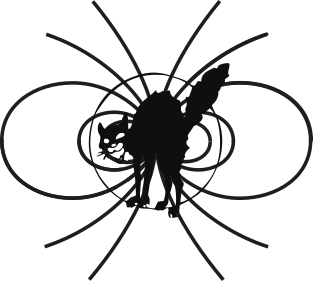
\includegraphics{images/cat3.png}
\caption{Wildcat in the field}
\end{figure}

\begin{figure}[htbp]
\centering

\includegraphics{images/elements.png}
\caption{Elements}
\end{figure}

\begin{figure}[htbp]
\centering

\includegraphics{images/squat.png}
\caption{Squat Sign}
\end{figure}

Some electrical symbols will also be incorporated, partly since many
things we will make involve building electrical circuits, and building
those symbols into the art makes things self-documenting. While these
form a useful function in helping to make a thing free by documenting
how it's put together, they should never abandon form for function:
circuit documentation should be a work of art as much as a document.

\subsection{Capitalisms Unwanted: a Human
Treasure}\label{capitalisms-unwanted-a-human-treasure}

One of the sources of constant pain for most people subject to global
capitalism is the phenomenon of some humans being simply unwanted by
capitalism. The people who live in the big cities and write computer
code for a living and control the nodes of power in our society no
longer have use for most of humanity. This is true even in a supposedly
``rich'' country like the United States or France. Looked at globally,
whole nations are written off by the global elite as disposable, a mere
nuisance. Meanwhile, war, an inevitable aspect of capitalism, creates an
endless stream of people who have had even what little shreds of social
wealth they might have had smashed by the war machines of Capital.
Environmental destruction will also create increasing numbers of
refugees as population grows and our living world continues to be
murdered by Capitalists.

The people in this ``unwanted'' demographic have nothing to gain from
the current system. Most of the laws in our system exist to protect
property owners from those who do not have property. As long as someone
owns property, the capitalists care at least enough about them to tax
them. Once someone has no property \emph{and} no special technical
skills to put them in the priesthood of ``tech'' the capitalist system
has zero use for them and thus doesn't bother to help them even survive
any more than they have to as vestiges of the society the Reaganists
have destroyed in the last 40 years.

But from our standpoint the concept of a ``lower class'' simply makes no
sense. Each human mind has infinite power to create art and science and
culture. The fact that capitalism has created an infinite stream of
unwanted humanity outside their system, who have zero vested interest in
that system simply means there is an unlimited supply of human genius to
deploy on post capitalist projects. The future belongs to those who are
able to welcome capitalisms unwanted with open arms as the infinite
treasure they are rather than constantly attempting to cull out the
``unwanted'' from their own ranks, driving the working poor out of their
cities or off their land.

We must develop technology/art/culture which naturally appeals to and is
instantly useful to those abandoned by capitalism. It's the right thing
to do, since they are the most underserved in the current system. But
it's also the long term strategic thing to do, since it means we will
naturally out grow and overtake the capitalist system as we build
something that is better enough that more and more strata of the
existing society jump across to the free world and join us.

\subsection{Skeletron: The Wooden Bones of
Art}\label{skeletron-the-wooden-bones-of-art}

Skeletron is the system that makes the bones of Trash Magic artifacts.
Skeletron is simply a way to modify things found in your environment to
make them play together well with Trash Magic. Primarily this means
gathering sticks, shaving them to be flat on one or more sides and
removing the bark, and drilling holes in them. Quarter inch holes spaced
about one inch along the line of the sticks is the most basic component
of Skeletron. This can be used to do many things, and as more people
build it and use it and modify it, it will become increasingly versatile
and free.

With a universal wood framing system we can build up many different
human sized structures. This can be used to make various shelters,
although to do this we will add plastics to the system, using methods of
hand plastic welding detailed in the last chapter of this volume. With
the ability to make wood skeletons with plastic skins we can make
waterproof structures on land as well as waterproof boat structures and
amphibious artifacts of various kinds. The combination of wood and
plastic in a modular and modifiable way also can be the basis of all the
other industrial constructions to be described in this work.

\subsection{Trash Magic Kit: The
Stickening}\label{trash-magic-kit-the-stickening}

Part of practicing Trash Magic is having constant access to some basic
technology kit, generally based on various sticks from the above system,
which can be used to build up everything else.

What are some capabilities of Trash Magic kit?

\begin{enumerate}
\def\labelenumi{\arabic{enumi}.}
\tightlist
\item
  Measuring tools: distance, position, mass, volume, temperature,
  pressure, etc.
\item
  Electrical to acoustic probes to measure the electrical properties of
  our environment in real time
\item
  Optical microscopy
\item
  Conversion to robot mode where it drives itself around
\item
  Convenient single shoulder strap for comfortable wear like a bike
  messenger pack
\item
  Music player
\item
  High voltage storage capacitors
\item
  Batteries for low voltage storage
\item
  free space optical audio communication(analog)
\item
  fractal fluid control
\item
  can harvest energy using a built in magnet and coil setup
\item
  water pump always available
\item
  goggles that can interface with various imaging technology using
  analog displays with vibrating fluids
\item
  3d imaging at all scales with vibration of fluids and ion transport
\end{enumerate}

\subsection{Free Phones in Trash
Magic}\label{free-phones-in-trash-magic}

One of the many idiotic things capitalists say to shut up their critics
is to point out that capitalism is the source of the smart phones that
anti-capitalists inevitably use. These devices are indeed amazing, and
are no longer luxury items by any means. On the contrary, they are very
much a survival tool used by the oppressed classes now, and it's very
dangerous to ignore that role this technology plays. But what aspect of
them is so great? The social networking. That's always what you need:
access to the web, various messaging systems, and various commercial
things like Uber and Lyft.

Does that really need to be a computer? A truly free phone would be a
pure communication tool that communicates in a distributed way like fido
net of old. the sole purpose of the hardware would be to communicate
images, sounds, text, and to decide where those should go. That's it.
What the hell do you need a computer for? Mostly so that The Man can spy
on you and figure out how to sell you things you don't need, and force
you to constantly throw more federal reserve debt back into the machine
for more advanced machines to get more indoctrination to continue the
cycle.

Don't be fooled by the dominance of the computer technology into
believing that's inevitable. It's not. We can get orders of magnitude
more benefit from peer to peer networks than we do today as slaves to
the military industrial machine if these phones were all free like
freedom, linked up on free hardware all the way. This can actually be
the basic informational skeleton of the value circles.

I believe that the hardware can be re worked from the ground up based on
our approach to applied electromagnetism to get something with totally
new fab. But in the mean time, given that that is a lengthy applied
physics research project, what can we do? My answer is to watch closely
everything that has anything to do with Raspberry Pi and other
``internet of things'' projects in the open hardware domain. I say
``open hardware'' here and not free hardware, because it's not free
according to my strict definition: it relies on mine- driven fab and
capitalism, and there is IP in the supply chain(and some other
problems). But it's way better in terms of open and free than the whole
android/apple ecosystem.

\subsection{The Tripod and Multitool}\label{the-tripod-and-multitool}

The basis for all Trash Magic fabrication will be the tripod. a tripod
is exactly what it sounds like: three sticks, joined at the top with
wire or tape or rope, as well as with guy wires at the bottom if needed,
with the bases of the three sticks planted in the ground for stability.
A rock hangs from the center to keep it steady.

Each of the three sticks shall be of Skeletron. Each shall be the size
of the Standard Trash Magic Staff. A practitioner of Trash Magic shall
have the power to deploy this at any time, at any scale and with any
tool. Full xyz motion is possible with wires that are fed through holes
or wheels on the sticks, and can go to stepper motors for drive and/or
wheels on potentiometers. Each wire connects to an arduino that runs a
three terminal pulsed transport measuring protocol. The ADC signals are
amplified and converted with some math to an audio signal, visual
display, and or vibrotactile interface.

This probe can be heated with the wires, can do local electrochemical
work and measurement, measure nonlinearities of all kinds, and can thus
weld, plate, edit, implant ions, plastic weld and plastic re-shape,
signals also displayed in a GUI in a smart phone if needed but can also
not be, can have no ``smart'' computer at all, just dumb computers.
Sensing can be capacitive, inductive, resistive, frequency dependent or
not, nonlinear or not, gated or not. Many different sizes and weights
can be used, gear ratios can be changed on the fly with various
interchangeable wheels. Everything is modular.

Thermal regulation of processes can be carried out by moving the
position of a suspended cauldron in 3 dimensions relative to a fire at
the bottom of the tripod, using a microprocessor and feedback on a
thermometer to regulate the temperature to a fixed point.

In a cluster of Trash Magic industrial production there can be many
tripods, all in a network, connected by plastic plumbing, electrical and
data connections, and zip lines that move materials from one to another,
setting up ad hoc nodes in an assembly line that can be grown and shrunk
on the fly.

Tripods can also support roof and wall materials, making shelters that
people can sleep and work in. Tripods can be trees that already exist.
Tripods can also be completely submerged for doing intricate work on the
bottom of a body of water. In zero gravity another set of sticks are
needed, and another cable and springs. The materials for a pair of
tripods should also be able to become the skeleton of a simple boat,
which can then deploy mini tripods to the water below it.

Tripods can be fractal, with a small tripod lowered from the tool head
of a large tripod. Smallest tripods should have Angstrom resolution and
atomically sharp tips, biggest ones are hundreds of meters tall.

\subsection{\ldots{}And More}\label{and-more}

This chapter is one that must be sparse in the first edition but which
will expand in the future. That is because I have a bit of a chicken and
egg problem: I need a finished manifesto to inspire me into total
commitment to the applied physics research, but need the fruits of that
research to properly deploy this first edition manifesto. So I'll
attempt to split the difference here, just sketching out a crude shadow
of the things I plan to build, with the understanding that it's probably
wildly inaccurate based on how the research will create surprises.
